%reset references counter
\setcounter{NAT@ctr}{-1}
\cleartorightpage
\chapter*{}\label{chapter:phages}
\phantomsection\addcontentsline{toc}{section}{Phage Annotation}

% \begin{figure}[t!]
% \centering
% 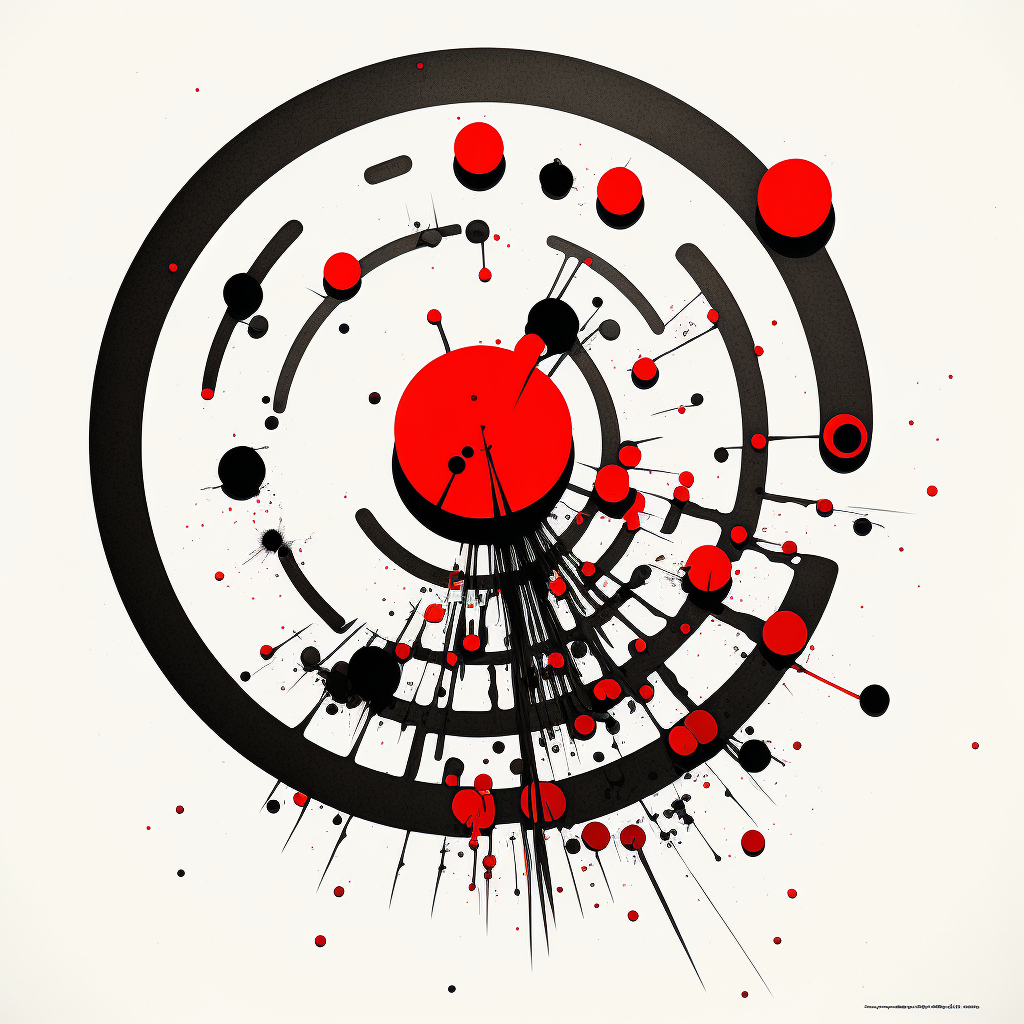
\includegraphics[height=10em]{chapters/phages.png}
% \end{figure}
% \vspace{-4cm}

\begin{changemargin}{0cm}{2cm}
\articletitle{Galaxy and Apollo as a biologist-friendly interface for high-quality cooperative phage genome annotation}
\end{changemargin}

Helena Rasche\textsuperscript{\ref{phage-affil:1},\ref{phage-affil:2}§},
Jolene Ramsey\textsuperscript{\ref{phage-affil:1},\ref{phage-affil:2}§},
Cory Maughmer\textsuperscript{\ref{phage-affil:1},\ref{phage-affil:2}},
Anthony Criscione\textsuperscript{\ref{phage-affil:1},\ref{phage-affil:2}},
Eleni Mijalis\textsuperscript{\ref{phage-affil:1},\ref{phage-affil:2}},
Mei Liu\textsuperscript{\ref{phage-affil:1},\ref{phage-affil:2}},
James C. Hu\textsuperscript{\ref{phage-affil:1},\ref{phage-affil:2}\dag},
Ry Young\textsuperscript{\ref{phage-affil:1},\ref{phage-affil:2}},
Jason J. Gill\textsuperscript{\ref{phage-affil:1},\ref{phage-affil:3}},

\textbf{Published in:} \emph{PLOS Computational Biology}, November 2, 2020 \\

\doi{10.1371/journal.pcbi.1008214}

\small

\begin{enumerate}
\itemsep-0.5em
\item Center for Phage Technology, Texas A\&M University, College Station, Texas, United States of America.\label{phage-affil:1}
\item Department of Biochemistry and Biophysics, Texas A\&M University, College Station, Texas, United States of America.\label{phage-affil:2}
\item Department of Animal Science, Texas A\&M University, College Station, Texas, United States of
America.\label{phage-affil:3}
\end{enumerate}

§ These authors contributed equally to this work.
\dag Deceased


\section*{Introduction}

Bacteriophage, or phage, are the viruses of bacteria. Their study
cracked open critical concepts in genetics, and allowed detailed gene
mapping before genome maps could be generated with ease \cite{Ofir_2018,Salmond_2015}. While
phage genomes were the first to be sequenced in their entirety, phage
research declined considerably before sequencing technologies took off.
Researchers from disparate fields in the modern age have come to a new
appreciation for the potential that phage have to help solve current
problems, as well as the commensurate challenges facing their
application \cite{Young_2015}. Scientists around the world are collecting phages
for a diverse panel of bacterial hosts that are relevant for the clinic,
in industry, and as model organisms. One stated intent is to establish
organized repositories, or phage banks, as a community resource for
their distribution \cite{Pirnay_2018,Pouillot_2010}. Coupling this with a surge in use of phage
for education and research training, an incredible boom of phage
sequencing has also emerged, with great promise for extending our
understanding of fundamental phage biology \cite{Hatfull_2011}.

The great sequencing explosion has resulted in many new viral \cite{Brister_2014}
and phage genomes being deposited into online databases. Because these
genomes are small, we can have high standards for complete, confirmed
contigs, and high-quality structural and functional annotation.
Unfortunately, many of the tools available to accomplish this task are
command-line based. When tools available for annotation run on the
command-line, they are not accessible to many biologists. Even if they
are, the output is not visual, integrated, or contextualized, and
requires much outside analysis. NCBI has released a suite of
command-line interface tools for (eukaryotic) virus annotation recently
\cite{Shean_2019}, and new phage-specific annotation pipelines are command-line
based making teamwork less fluid \cite{Ecale_Zhou_2019}. While the capability to do the
needed analyses is there, it is still out of reach for many teams. A
great need in the field is therefore to have easy-to-use, web-based
tools with a graphical user interface for annotation and community
annotation platforms to improve quality and promote shared input on
phage assessment for use in any given application. Because phages are
being rushed into application in humans for phage therapy without
measured and thorough safety checks put in place, many others agree that
manual inspection for high-quality annotation is needed \cite{Philipson_2018}. The
Center for Phage Technology (CPT) at Texas A\&M University has harnessed
two powerful online platforms to solve this problem.

\section*{Methods}

\subsection*{Galaxy \& Apollo at the CPT}

The Galaxy Project is a web platform suitable for beginner and advanced
biologists to perform analyses on biological sequence data \cite{Afgan_2018}.
Apollo is a browser-based, evidence-driven, and community-focused genome
annotation editor based on the popular JBrowse genome viewer
\cite{Lee_2013,Dunn_2019}. The CPT created a Galaxy-Apollo bridge to link the powerful
sequence analysis capabilities of Galaxy with the evidence-based
community annotation platform of Apollo to provide a complete
environment for the analysis and annotation of phage genomes
(\protect\hyperlink{pcbi.1008214.g001}{Fig 1}) \cite{Skinner_2009}. To date, more
than 120 phage genomes have been annotated using this platform and
publicly deposited (see NCBI BioProject
\href{https://www.ncbi.nlm.nih.gov/bioproject/?term=PRJNA222858}{PRJNA222858}).
Documentation on the CPT's Galaxy-Apollo phage annotation pipeline,
written at a level suitable for teaching undergraduates, accompanies the
CPT resources at \url{https://cpt.tamu.edu/training-material/}, with new
tutorials added regularly.

\begin{figure}
\hypertarget{pcbi.1008214.g001}{%
\centering
	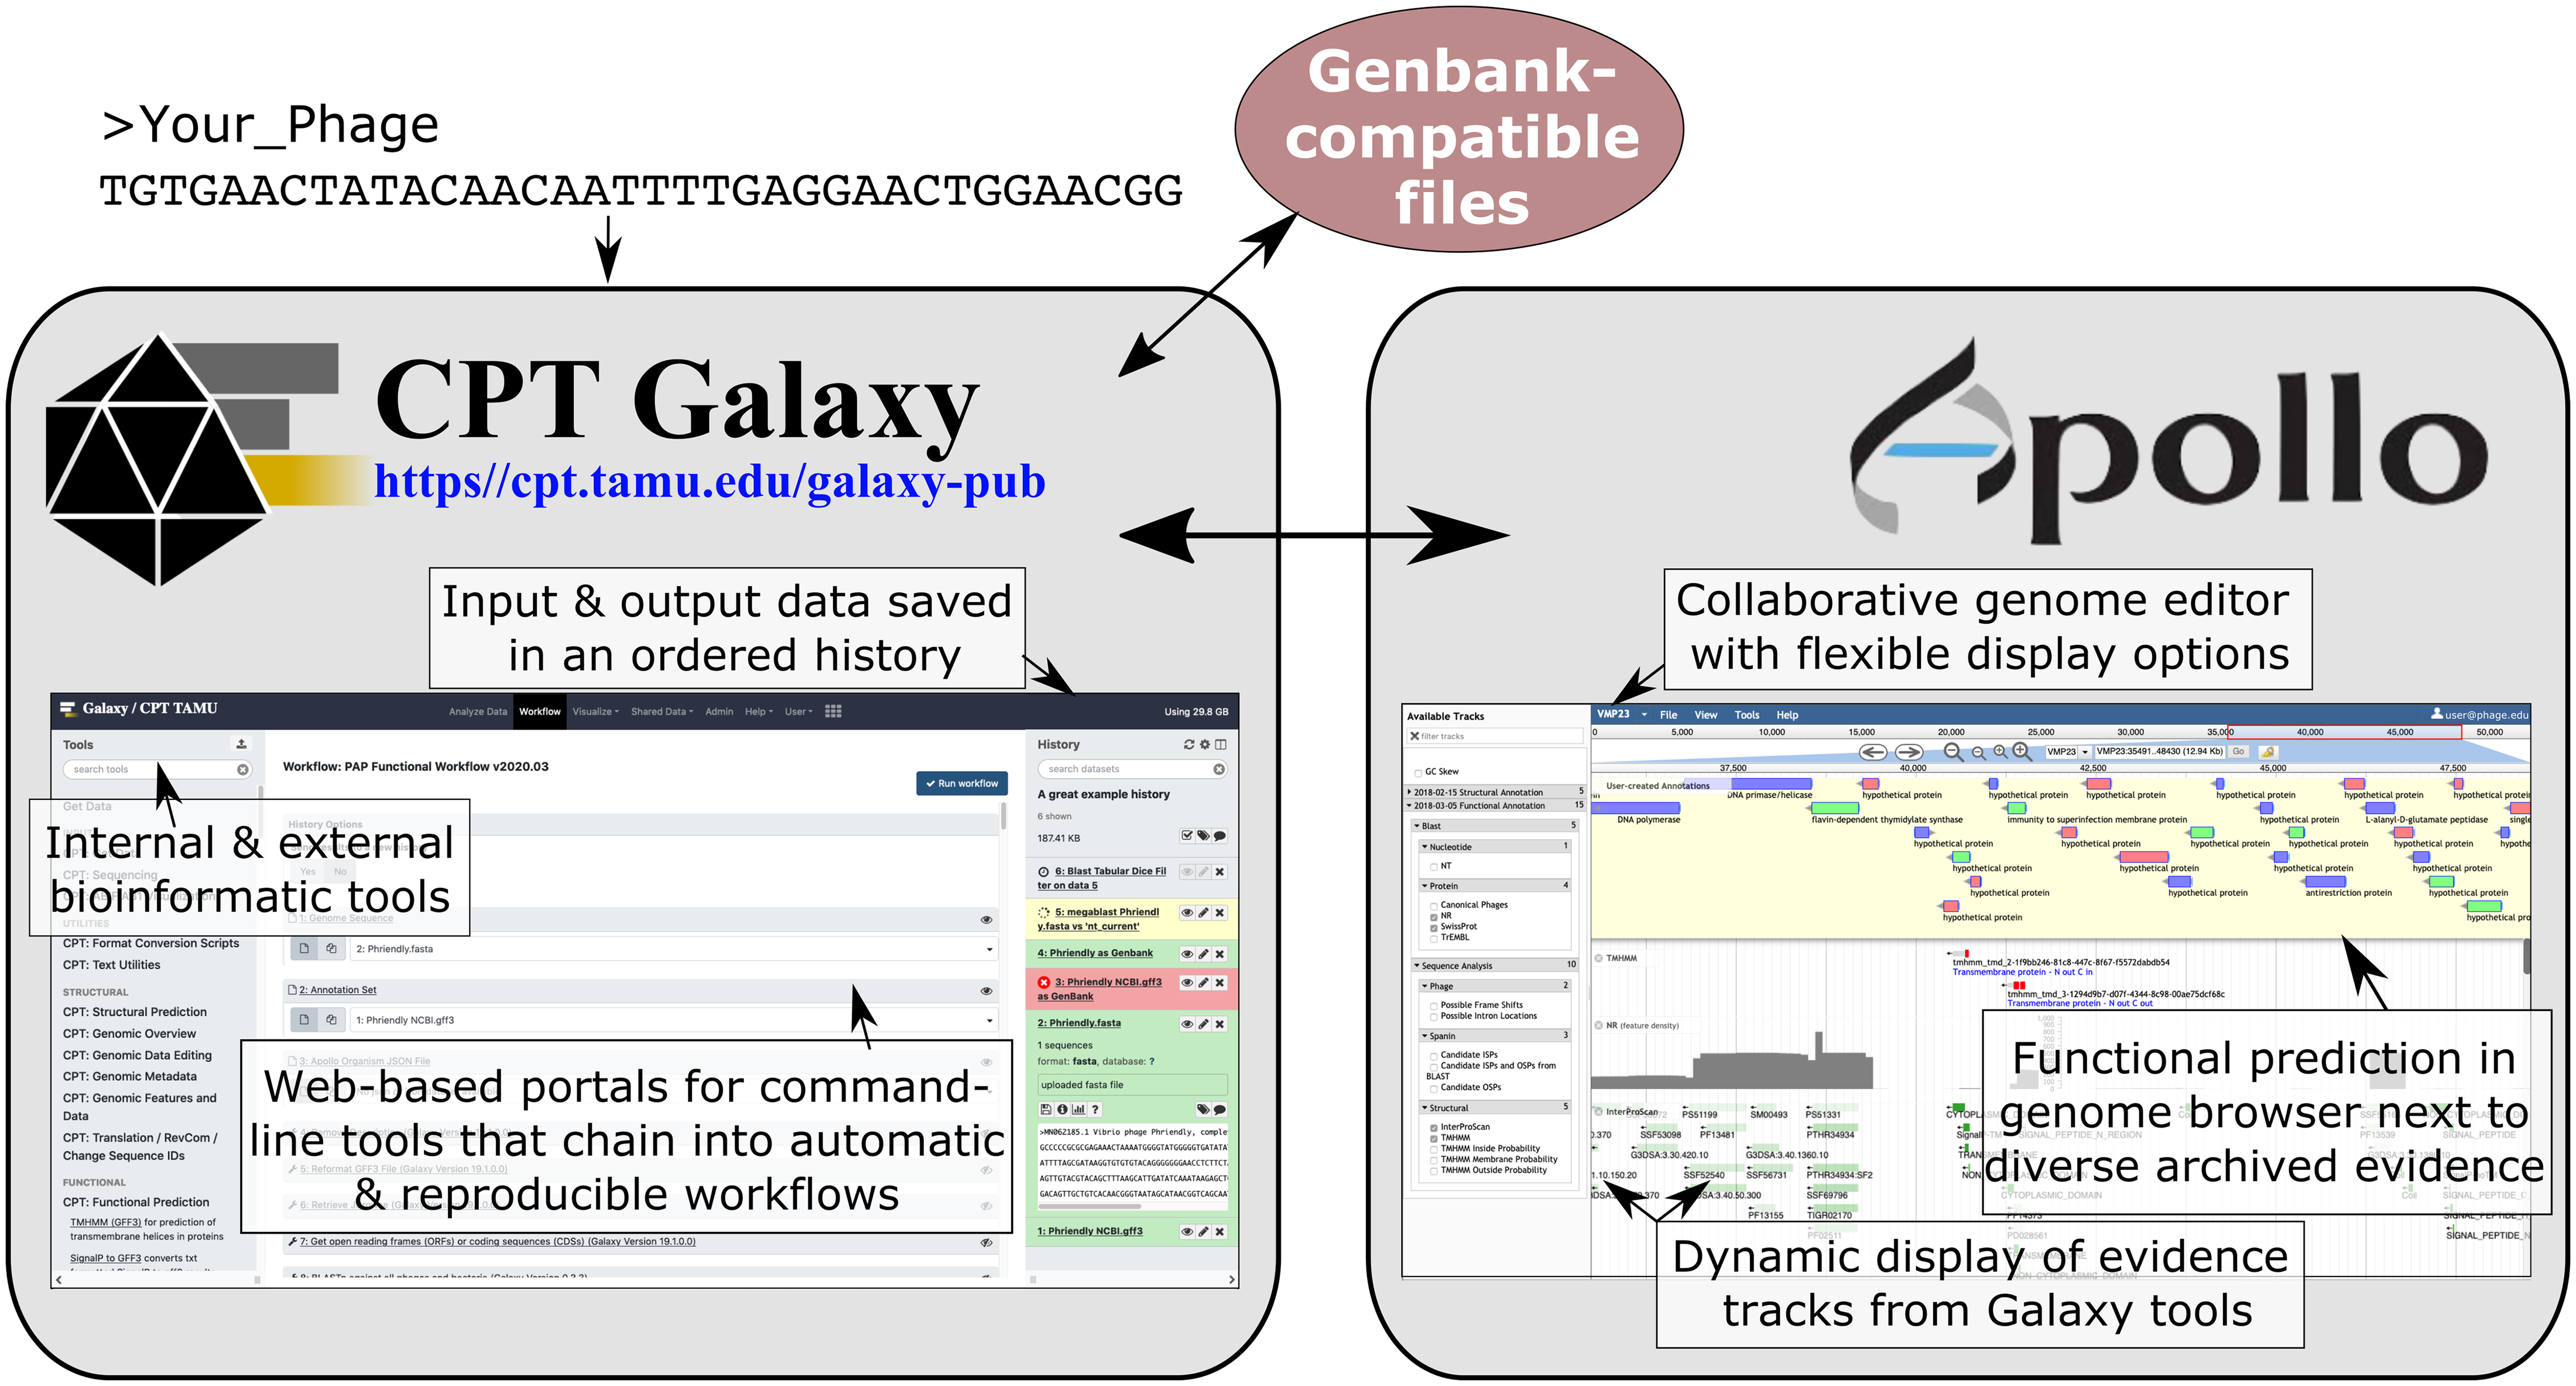
\includegraphics[width=\textwidth]{chapters/images/phages/1.png}
\caption{The Galaxy and Web Apollo interface used for analyses and
annotation.\\
By coupling the Galaxy platform for analyses with the editing
capabilities in Apollo, contextualized evidence can be used to
iteratively annotate genomes as a team effort.}\label{pcbi.1008214.g001}
}
\end{figure}

\subsection*{CPT Galaxy, a flexible web-based platform for computational
analyses}

The major benefit of Galaxy as a bioinformatics platform is that it
allows traditionally-trained biologists to perform, record, and
visualize complex analyses on their own data within a browser-based
graphical user interface, rather than at the command-line. Researchers
spend their time analyzing the biological implications of results,
rather than troubleshooting the execution of scripts or managing files
at the command-line. Crucially, the browser-based interface makes the
system accessible to the common scientist. A second powerful feature of
Galaxy is the ability to chain tools together in workflows that run jobs
(the equivalent of a computational experiment) automatically, which
makes the system convenient for programmers and bench scientists alike.
Local or worldwide project administrators maintain the system operation,
update tools, and provide user support.

Detailed descriptions of Galaxy functionality are provided by the
developers, and here we give only a few highlights pertinent to our
discussion on its use for phage annotation \cite{Afgan_2018}. The user interface
in Galaxy revolves around three main panels where the work is ordered
(\protect\hyperlink{pcbi.1008214.g001}{Fig 1}). Tools, or bioinformatic
scripts, for data analysis are cataloged and searchable in the left
panel. The center Data Analysis panel provides a point-and-click
atmosphere for setting job parameters and viewing data. The right-hand
panel visualizes the stored history of each user analysis, which enables
good documentation and promotes reproducibility. Galaxy histories, akin
to a digital notebook, can be shared among users.

The standard Galaxy installation comes with tool sets contributed by the
scientific community, and can be expanded through tools available in the
ToolShed, by adapting open-source tools for the Galaxy interface, or by
writing new scripts to suit specialized analysis needs \cite{Blankenberg_2014,Cock_2013,Cock_2009}. The
CPT Galaxy instance offers various phage-specific tools described below
and a comprehensive selection of curated BLAST databases, including
SwissProt, NCBI nt and nr, as well as certain custom databases \cite{2018}.
A common challenge in using a large collection of tools from different
sources is the interoperability of the outputs. To facilitate moving
data output from one tool into the next, we have also gathered, adapted
or produced a comprehensive set of scripts that convert or parse various
tool outputs into standardized formats, including conversions between
tab-separated value (tsv), XML, Genbank, and GFF3 formats (see
\protect\hyperlink{pcbi.1008214.s001}{S1 Table} for partial list, search
at \url{https://cpt.tamu.edu/galaxy-pub} for full list).

\subsection*{Apollo at the CPT for teaching and crowd-sourcing advanced
phage genome annotation}

JBrowse is a widely-used, embeddable genome browser, capable of
displaying genome annotations and features from the level of the entire
chromosome down to the DNA sequence \cite{Buels_2016}. Apollo is a web-based
genome editor that builds upon JBrowse to provide the ability to do
persistent, manual genome annotation and curation inside an internet
browser window. Multiple users can view and/or edit the same organism,
resulting in Apollo being colloquially referred to as the `Google Docs'
for genome annotation. Whole genome and feature analysis results
conducted in Galaxy are displayed in tracks below their corresponding
locations in the genome, allowing the user to integrate multiple types
of evidence within genomic context when making annotations. The
centralization of evidence, especially within genomic context, makes the
view comprehensive and spares users from mentally integrating evidence
in disparate formats from multiple sources, a key achievement of the
system. A virtually unlimited number of evidence tracks can be added,
dictated primarily by the user's need for, and access to, additional
analysis types. Various forms of metadata can be added in both standard
and free-form entry methods, allowing rich annotation of each feature
within a genome. As needed, additional evidence from up-to-date analyses
in Galaxy can be added to the Apollo organism evidence tracks through
the Galaxy-Apollo bridge.

\subsection*{The Galaxy-Apollo bridge}

To meet the needs of reproducible phage annotation and scaling these
processes for the influx of new phage genomes, the CPT developed a
Galaxy-Apollo bridge. The bridge consists of a number of Galaxy tools
which interface directly with Apollo, enabling Galaxy users to move data
into Apollo, automate certain tasks within Apollo, and finally to
extract user-curated annotations back into Galaxy for further downstream
analysis.

During the annotation process, a user will create a JBrowse instance
within Galaxy, combining the genome and analysis results for
visualization. The \textbf{Create or Update Organism} tool sends this
data to Apollo either as a newly created organism in the Apollo system,
or as an update to an existing one. The \textbf{Annotate} tool uses the
output of the Create or Update step to provide an iframe window into
Apollo, permitting users to retain the context of their Galaxy analysis
history and tools, while allowing users to easily switch back to
interactive analysis. When manual curation is complete, users can run
\textbf{Retrieve Data}, to fetch the data from Apollo's `User-created
annotations' track into Galaxy. Tools including \textbf{GFF3 to Apollo
Annotations} and \textbf{Delete all annotations from an Apollo record}
enable significantly more automation between Galaxy and Apollo, and
future updates are working toward entirely automated annotation
pipelines. This set of tools bridges the two different worlds of Galaxy
and Apollo and tells one cohesive story: from DNA, to an annotated
genome, with the reproducibility of Galaxy and the freedom and real-time
collaboration of Apollo.

These tools inspired the Galaxy community to start the Galaxy Genome
Annotation project (GGA;
\url{https://github.com/galaxy-genome-annotation}/), resulting in the
development of a new Python library for interacting with Apollo, a
command-line suite for Apollo, and a new set of Galaxy tools generated
from the Python library.

\subsection*{Documentation available for new users}

To promote widespread adoption by biologists, step-by-step tutorials
with background for using Galaxy tools and the Apollo platform are
freely available at the CPT website:
\url{https://cpt.tamu.edu/training-material/}. Their format is based on
resources provided by the Galaxy Training Network \cite{Batut_2018}. Tutorials
are written at levels suitable for use by undergraduates learning how to
annotate phage genomes. The topics covered make them useful for the
scientist as well, including tutorials on phage genome assembly from
Illumina reads and instructions for polishing and depositing genomes in
the NCBI Genbank database.

\subsection*{Galaxy tools useful for phage annotation}

The customization of the CPT Galaxy instance is best understood as a
unified collection of tools that address the specific needs for phage
genome annotation; these tools are available for ad hoc usage or as part
of a workflow within Galaxy. The challenges associated with phage genome
annotation are inextricably linked with general prokaryotic annotation,
and intrinsically different from eukaryotic systems. Since intron
splicing is rare in prokaryotes and phages, and thus is not assumed
\emph{a priori}, tools in the CPT Galaxy are tailored to take advantage
of the fact that genes and protein-coding sequences can be called
directly from the DNA sequence. Furthermore, many features of the
pipeline described below could also be useful for annotating bacterial
genomes, although the larger size of bacterial genomes would benefit
from increased automation in certain procedures. Below, we describe the
development of resources motivated by gaps we experienced within the
available annotation tools and platforms.

\subsection*{Quality control of gene calling using ShineFind}

All phages rely on host machinery for translation, and as such their
genes typically have recognizable prokaryotic signals. The
Shine-Dalgarno (S-D) sequence is a component of the ribosome binding
site (RBS) situated upstream of the start codon in prokaryotic genes,
and its presence can serve as a strong indicator of gene starts.
However, gene callers with high-quality algorithms do not universally
include the ribosomal binding site when predicting the locations of
protein-coding genes. We wrote a stand-alone tool called
\textbf{ShineFind} to annotate S-D sequences as part of the standard
gene model in Apollo. This Python script accepts GFF3-formatted gene
calls and its associated FASTA DNA sequence file as inputs. ShineFind
then extracts the upstream sequence for all CDS features that do not
already have an RBS in their gene model; this defaults to extraction of
upstream nucleotides 3--24, but is editable by the user at runtime.
Those upstream sequences are then searched for matches to the \emph{E}.
\emph{coli} consensus S-D sequence AGGAGGT, or smaller subsets of this
sequence (see full list in \protect\hyperlink{pcbi.1008214.s002}{S2
Table}). By default, the longest match to the consensus is returned, but
all the smaller matches can also be output. The returned S-D match is
added to the GFF3 gene model as a child of the gene feature and named
``Shine\_Dalgarno\_sequence'' (a sequence ontology term \cite{Mungall_2011,Eilbeck_2005}),
and can then be displayed within Apollo. The consensus S-D sequence and
recognized subset sequences can be swapped for an alternate sequence set
by editing the Python script. GFF3 annotations that already contain S-D
annotations can be stripped of these features using the tool
\textbf{GFF3 Feature Type Filter}, which is also part of the Structural
Workflow described below.

\subsection*{Finding candidate spanin genes}

There are special cases among phage genes, such as the lysis genes,
which are difficult to detect by standard methods relying on simple
sequence similarity. The spanin genes needed for outer membrane
disruption during phage lysis of Gram-negative bacterial hosts are often
missed or mis-annotated, largely due to their unique genetic
architecture in which one gene is often embedded in an alternate reading
frame within the sequence of another \cite{Kongari_2018}. Spanins can function as a
single or two-protein system, but the proteins share the same
characteristics. The inner membrane spanin (i-spanin) contains a
transmembrane domain, whereas the outer membrane spanin (o-spanin) will
be cleaved and lipoylated by the bacterial lipoprotein processing system
at a Cys residue at the end of a lipobox motif \cite{Babu_2006,von_Heijne_1989}. Their varied
genetic architectures, particularly when the o-spanin gene is fully
embedded within the i-spanin gene, and clear domain signatures are keys
to the suite of tools that we have developed to find them \cite{Cahill_2019}.

To account for the fact that spanin genes are highly prone to be
uncalled or called with incorrect start sites, spanin-finding begins
with naïve ORF calling by the tool \textbf{Get open reading frames
(ORFs) or coding sequences (CDSs)} \cite{Cock_2013,Cock_2009} finding all possible ORFs
(using the NCBI translation table 11 for Bacteria and a 30 aa minimum
length cutoff), and generating an output in GFF3 format. The gene model
within the GFF3 file is corrected by the addition of a gene parent
feature to every CDS. The ORFs are then filtered to include only those
with a common phage start codon (ATG, GTG or TTG) and ShineFind is used
to add potential Shine-Dalgarno sites where they exist.

From there, the naïve gene sequences are translated and analyzed in
three ways. 1) Protein similarity to spanins in a curated database
\cite{Kongari_2018} is determined by BLASTp with a 0.001 expectation value cutoff.
2) Potential lipobox motifs expected for outer membrane spanins are
identified using the tools \textbf{LipoP} \cite{Juncker_2003} and \textbf{Identify
Lipoboxes}, a less stringent regex amino acid motif search for the
four-residue motif {[}ILMFTV{]}-{[}any residue except
REKD{]}-{[}GAS{]}-{[}C{]}, or {[}A{]}-{[}W{]}-{[}AGS{]}-{[}C{]}. 3)
Inner-membrane spanin candidates are identified through \textbf{TMHMM},
which predicts transmembrane regions \cite{Krogh_2001}. Finally, to reduce noise,
the results from Lipobox/LipoP and TMHMM predictions are cross filtered
to require putative inner- and outer-membrane spanin gene pairs occur
within 50 nucleotides of each other and be located on the same strand,
consistent with the architecture of known spanin genes \cite{Kongari_2018}.
Analysis using both explicit protein similarity by BLASTp and searching
for more general spanin signatures allows for the identification of all
spanin types and high-quality selection of likely start sites. This
approach was able to identify a test set of experimentally verified
spanins. However, the output needs to be critically assessed before
genes are confidently assigned spanin functional predictions; the
signature-based approach of identifying genes that pair with nearby
genes containing lipoprotein or TMD signals is prone to producing
multiple false-positive results in the average phage genome, as it
ignores genomic context and the presence of other genes. These
false-positive results can typically be excluded upon cursory
examination of the results due to their presence embedded within other,
obviously non-spanin genes. Additionally, drawing connections within
novel phages has allowed the computational identification of novel
spanin genes \cite{Kongari_2018}.

\subsection*{Identifying interrupted genes}

Several types of interrupted genes are present in phages, including
programmed translational frameshifts, introns or inteins. Researchers
typically use an integrated approach to detect the presence and
boundaries of expected interrupted genes. Because the functional
analysis performs sequence similarity searches, we can take advantage of
those results to identify interrupted proteins compared to their
uninterrupted counterparts present in the database. Due to biological
variety in this area and chain annotation that tends to propagate common
annotations (over quality annotations), much work is needed here to
populate the databases with accurate annotations. The \textbf{Intron
Detection} tool can detect legitimate introns (often in essential
genes), frameshifts or premature stops produced by sequencing errors
(such as those introduced by long-read sequencers), programmed
translational frameshifts (frequently found in capsid proteins or tape
measure chaperones), and other split or duplicate gene phenomena.

In the CPT Galaxy pipeline, the interrupted genes detection tool parses
XML-formatted BLASTp results to determine whether multiple query
proteins from the phage genome have amino acid identity to a single
target protein in the database. The presence of a single database
protein as multiple discrete segments in the query genome is the
signature of a gene disrupted by an intron, programmed translational
frameshift, or sequencing artifact. The tool requires that the separated
gene fragments in the query genome exist within a user-defined number of
bases, with the default set at 10,000. Separation minimum evaluates
overlap of queries on the subject sequence (in case gene calls with
incorrect starts were input); negative values allow overlap and
positive/zero values allow separation. Logical checks in the script
include removing alignments with high identity over a short part of a
longer segment (identities/hsp length\textless0.3 are discarded),
requiring at least two unique high scoring pairs for any given target,
and ensuring that the common hits are encoded on the same strand. This
tool can also detect separated genes that span the genome ends, for
cases where a genome may circularize or if it is opened in the middle of
a gene.

In the case of introns, which are self-splicing RNAs usually found in
essential genes, they share common secondary RNA structure but are not
commonly predicted as part of annotation pipelines unless they contain a
well-known intron-encoded protein. Studies have shown that
\textasciitilde25\% of bacteria contain genes with group II introns,
while phage regularly contain group I introns \cite{Lambowitz_2010,Candales_2011,Leclercq_2012}. In the case
of T4 and T4-like phages, these mobile elements are seen to vary
substantially \cite{Edgell_2010,Petrov_2006,Petrov_2010}. The most reliable way to find the true
boundaries is by manual inspection of high-quality alignments of the
intron-disrupted phage protein segments against a non-interrupted
homolog from the database, which is identified in the tool output in
Apollo. When uninterrupted analogs do not exist in the database, or the
nearest uninterrupted analog has weak sequence identity, boundaries
cannot be accurately determined bioinformatically.

There are several kinds of important proteins in phages that are
produced via programmed translational frameshifting mechanisms, such as
the capsid or tail proteins and the tail tape measure chaperones, of
which λ is the best characterized example \cite{Baranov_2006,Atkins_2016,Xu_2004,Garci_a_2004,Auzat_2008,Condron_1991}. When the
frameshifted downstream open reading frame of a protein has been called
as a separate protein-coding gene (often without a strong SD), it can be
detected by the interrupted genes tool. However, in cases where no
experimental data exists for the matched protein in the database, the
potential for an interrupted gene should be interpreted with caution.

Finally, the interrupted genes tool can be very helpful for interpreting
long reads with many errors, such as those that result from nanopore
sequencing. Taking into consideration the noisy output of gene calling
(reducing stringency for ORF length and starts), this will be most
successful where the genome has high similarity to previously deposited
genomes.

\subsection*{Custom BLAST databases and BLAST restriction by TaxID}

The mainstay method for sequence comparison in genome annotation is
BLAST \cite{Camacho_2009}. While the number of sequenced phage genomes present in
the NCBI database has increased rapidly since next-generation sequencing
became widespread \cite{Hatfull_2011,Merrill_2016}, so have sequences of cellular organisms
and eukaryotic viruses \cite{O_Leary_2015}. Sequences outside bacteria and phages
are usually not relevant to our analyses, drown out low similarity hits
of interest, and significantly increase required processing time. The
CPT Galaxy instance, with locally installed database copies updated
about three times per year from their respective home sites, offers at
least two ways to mitigate those weaknesses: custom databases and
restriction by TaxID.

\emph{Custom databases}. Users can generate their own local databases in
Galaxy (via the \textbf{NCBI BLAST+ makeblastdb} tool), or use public
databases pre-compiled by the CPT. Significantly, we offer a `Canonical
Phages Database', representing the proteomes of phages with significant
publication history or of historical importance. This list includes
paradigm phages such as Lambda, T4, and T7, as well as P22, P2, and
phi29 (see \protect\hyperlink{pcbi.1008214.s003}{S3 Table} for full
list). The reason for generating this custom database is to ensure that
those phage proteins annotated based on experimental evidence are
detectable as hits against novel phage proteins, rather than them being
lost amid a slew of less relevant results. This ensures that when there
is a single degree of separation between the predicted protein of a
novel phage and a studied protein in a canonical phage, that prediction
can have higher confidence.

When analyzing phage genomes for therapy applications, toxin/anti-toxin
systems, restriction-modification systems, CRISPR-related proteins, and
anti-CRISPR proteins are of particular interest to detect. Despite wet
bench experiments being performed on many of these proteins, they are
poorly annotated in most databases. Custom databases from users or the
community can be added to Galaxy for specialized analyses.

\emph{Restriction by TaxID}. In the \textbf{BLAST+ 2.9.0} suite using
version 5 databases, standalone BLAST jobs can now restrict searches by
TaxID, as has long been available on the NCBI BLAST webserver. On the
CPT Galaxy instance, we modified the BLAST wrapper to make this
functionality available, with searching using non-species-level IDs
available with the TaxonKit tool to retrieve all species-level TaxIDs
that are required by BLAST 2.9 \cite{Shen_2019}. Using curated lists of TaxIDs
that include all phages, bacteria, and/or canonical phages
(\protect\hyperlink{pcbi.1008214.s003}{S3 Table}), we are able to
drastically reduce the processing time while targeting searches more
effectively.

\subsection*{Additional tools}

In CPT Galaxy, there are also assembly tools, including \textbf{SPAdes}
and \textbf{FastQC}. Since phage genomes are relatively small, typically
\textless200 kb \cite{Dion_2020}, they usually assemble completely in a single
contig that is opened randomly by the assembler. Biologically, phage
genomes can have physical ends with or without terminal repeats, or be
circular \cite{Merrill_2016}. As with other genome browsers, wraparounds are not
supported at this time in Apollo. Therefore, the genome is displayed
linearly and users must exercise careful judgement on interpretation of
all features that border or span the boundary of unannotated genomes.
Relatively few phages have had the state of their physical genomic
termini probed. Therefore, we rely on comparisons to phages with
empirically verified ends and computational predictions, whose
accessibility is limited by the specific sequencing technology used.
\textbf{PhageTerm} is an end prediction program installed in CPT Galaxy
\cite{Garneau_2017}. These software assessments can be useful in determining the
most logical place to re-open a genome, usually decided by convention in
the field. \textbf{Genome Editor} is a tool that allows rearrangement of
the genome, with or without associated annotations. There are also tools
that extract subsets of data from various genome record file types,
validators to check their format, and a \textbf{PhageQC} report
generator, useful for reviewing the quality of external genome
annotations. For those accustomed to or desiring an external tabular
file that collates their annotation data, the \textbf{Annotation Table}
tool generates a downloadable Excel-compatible table. These, and a whole
suite of plain text, table, and protein/nucleic acid manipulation tools
are searchable at \url{https://cpt.tamu.edu/galaxy-pub/}.

After all desired analyses are completed, the logical next step is to
deposit the sequence with its annotations into one of the public
sequence repositories. The tools to retrieve the data from Apollo into
Galaxy, as well as interconvert between file types, aid in this
essential step. The \textbf{Retrieve Data} tool yields a DNA FASTA file
and GFF3 file. These can be converted into a Genbank file with the
bacterial (default) translation table qualifier added using the
\textbf{GFF3 to Genbank} tool, then into the 5-column table used with
NCBI's BankIt service using the \textbf{Genbank to Five Column Format}
tool. Updates and new tools are regularly added to the CPT Galaxy
platform. The most current development version is available through our
public Github at (\url{https://github.com/TAMU-CPT/galaxy-tools}).

\subsection*{Workflows in Galaxy facilitate efficient multi-step analyses required for phage genome annotation}

While having all these tools in one place is useful, the human hours
required to sit at the computer and manually move the output from one
tool into the next, and converting those files into compatible formats
along the way, is prohibitive. We prefer to spend our time on the things
that computers cannot do as well: making judgment calls on the
annotations. Galaxy workflows offer the ability to chain many tools
together automatically, such that a long and tedious analysis can be
reproducibly applied to multiple datasets with a few clicks. Three main
workflows are the mainstay of our phage annotation pipeline: the
Structural Annotation workflow, the Functional Annotation workflow, and
the Comparative Genomics workflow. Using the tools described above and
in \protect\hyperlink{pcbi.1008214.s001}{S1 Table}, analysis is
conducted in Galaxy and then transferred to Apollo via the Galaxy-Apollo
bridge, where evidence is displayed for interrogation by the user, who
has ultimate control over the annotation process.

\subsection*{Structural annotation workflow}

The purpose of the structural workflow is to provide the researcher with
the evidence needed to make high-quality, confident gene calls with
accurate prediction of the gene start. This is accomplished in 23 total
steps from input genome FASTA file to the updated Apollo organism with
evidence tracks (\protect\hyperlink{pcbi.1008214.g002}{Fig 2}). The
structural workflow is relatively quick for phage genomes, usually
taking \textless20 minutes to complete.

\begin{figure}
\hypertarget{pcbi.1008214.g002}{%
\centering
	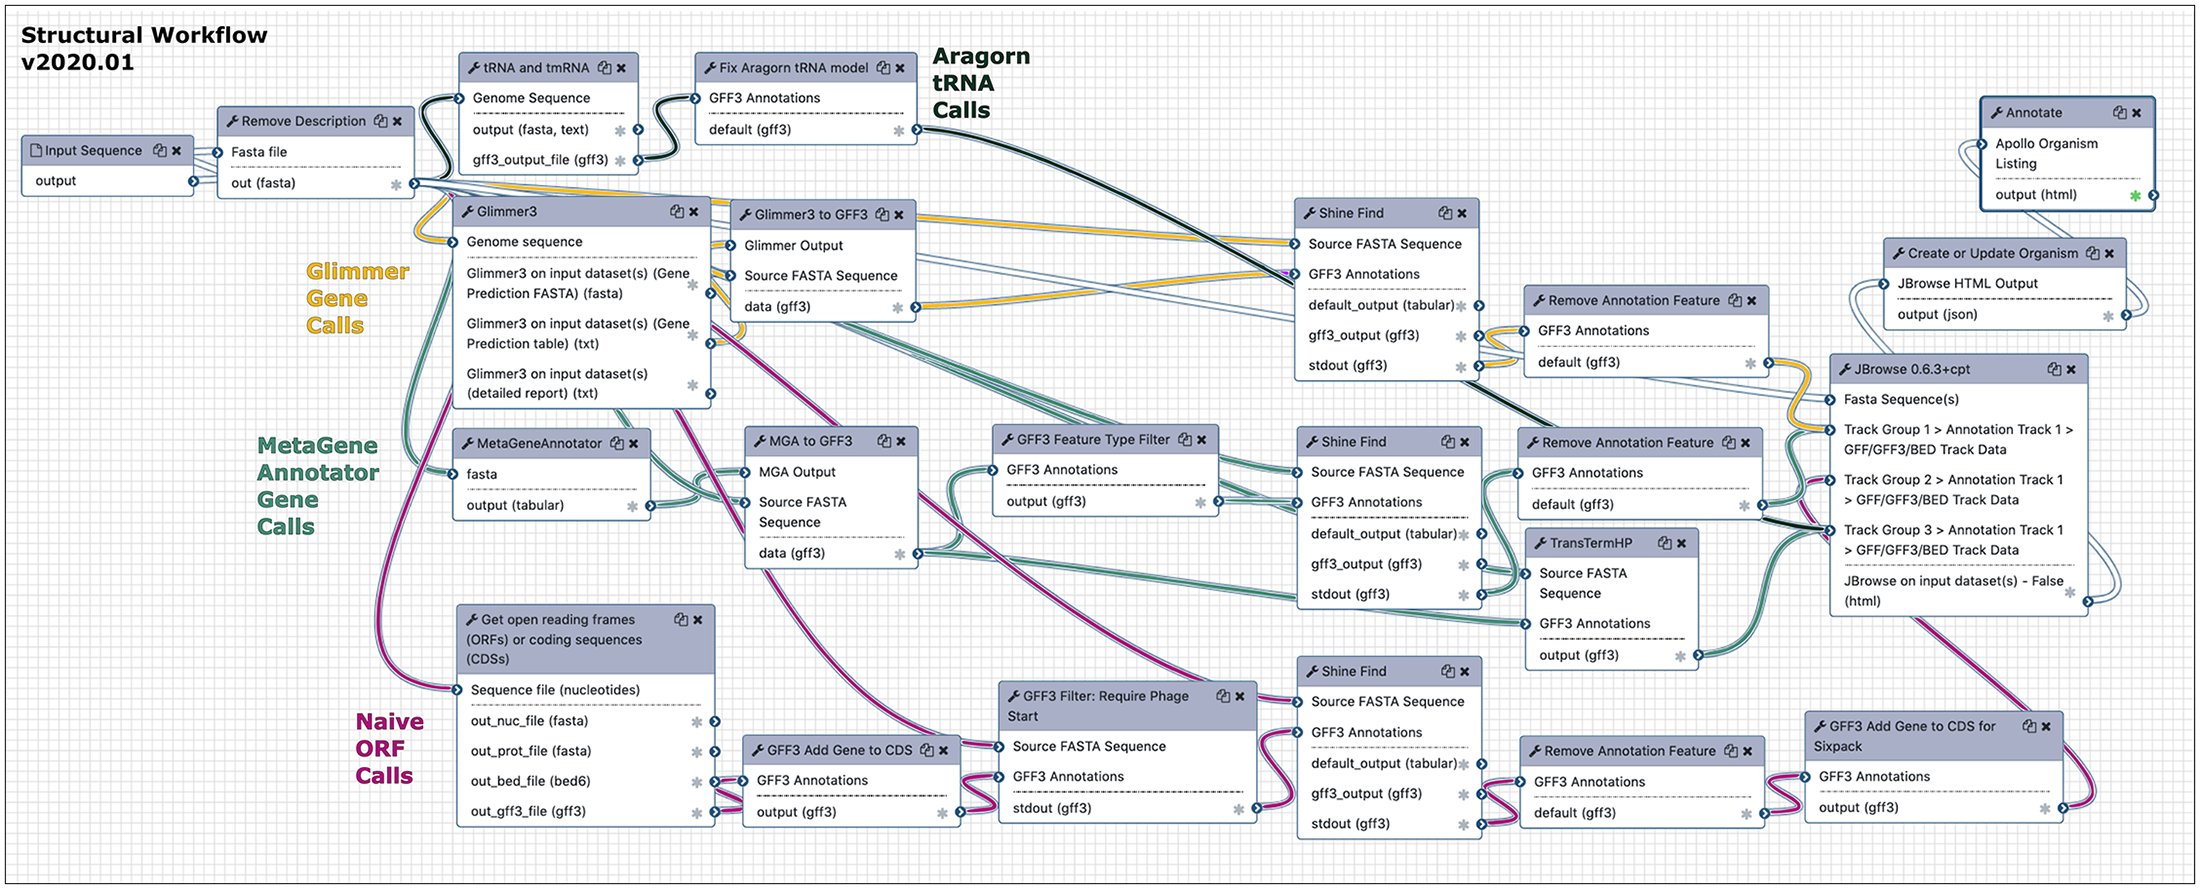
\includegraphics[width=\textwidth]{chapters/images/phages/2.png}
\caption{The structural workflow chains together tools in Galaxy for
gene calling.\\
The structural workflow accepts as input a nucleotide FASTA genome
sequence, and processes it through ARAGORN for tRNAs (dark noodles),
Glimmer and MetaGeneAnnotator for high-confidence gene predictions
(golden and teal, respectively), and Get ORFs as a naïve ORF/CDS caller
(magenta). Potential protein-coding genes are filtered to ensure the
presence of a phage (ATG/GTG or TTG) start codon and a Shine-Dalgarno
feature is added to all features that have a detectable match. These are
interconverted between formats and the gene models are corrected for
display in Apollo.}\label{pcbi.1008214.g002}
}
\end{figure}

From the naked input DNA sequence, five separate gene analysis tracks
are initiated. Two gene callers, \textbf{GLIMMER} 3.0 and
\textbf{MetaGeneAnnotator} v1.0 (MGA), both popular prokaryotic
prediction programs, are used to predict the locations of protein-coding
genes \cite{Delcher_1999,Noguchi_2008}. Their outputs are converted into GFF3 format and
processed by ShineFind; RBS sequences assigned by MGA are discarded
(feature filter step) in favor of the ShineFind algorithm. The outputs
are then properly formatted with a gene model structure that follows
gene-CDS and gene-Shine\_Dalgarno parent-child relationships for display
as a feature track for JBrowse. The MGA gene calls are used to predict
rho-independent transcriptional terminators using \textbf{TransTermHP}
\cite{Kingsford_2007}. A third gene caller, \textbf{Get open reading frames (ORFs) or
coding sequences (CDSs)}, uses the Sixpack framework from EMBL, preset
to use the NCBI translation table 11, for minimum 30 aa long ORFs with
both a start and stop codon \cite{Cock_2013,Cock_2009}. The GetORFs output is further
filtered to only genes with phage start codons (ATG, GTG, and TTG) along
with reformatting the gene model before formatting for display as a
feature track for JBrowse. tRNA and tmRNA genes are predicted by
\textbf{ARAGORN} v2.36 and also formatted for display as a feature track
in JBrowse \cite{Laslett_2004}.

Phage genomes are highly compact due to packaging constraints imposed by
the amount of genomic DNA or RNA that can fit into the capsid
\cite{Miller_2003,Kang_2017}. With a typical \textgreater90\% coding density,
protein-coding genes often overlap by several bases with adjacent coding
sequences. Many overlapping genes are missed by gene calling algorithms
trained on bacterial genomes which are not subjected to compaction
\cite{Kang_2017,McNair_2019,Akhter_2012}, which is why the CPT Galaxy pipeline is designed to allow
comparison of the results from three programs. MGA and GLIMMER results
usually agree, and predict the majority of protein-coding genes in the
genome. However, when gaps are present, they can often be filled by
reading frames identified in the naïve (and noisy) GetORFs/Sixpack
track. The user may evaluate the tool outputs and determine which
predicted genes are promoted to protein-coding gene features in the
Apollo editor window. As ARAGORN only displays tRNA predictions of high
confidence, these are typically all promoted as features. The
TransTermHP results are evaluated by the user, and may be promoted as
annotations based on the criteria of a score \textgreater95, a hairpin
stem with at least 5 matches, a minimum four-T run in the T-tail after
the stem, and genomic context. These annotations can then be imported
back into Galaxy as a GFF3 file for further analysis.

\subsection*{Functional annotation workflow}

The goal of the functional workflow is to provide the user with
contextualized evidence to predict the function of the proteins encoded
by their input genes. The 57 steps comprising the functional workflow
are the main workhorse of the phage annotation process
(\protect\hyperlink{pcbi.1008214.g003}{Fig 3}). Due to the use of BLAST
and InterProScan, the functional workflow can take several hours to
complete, commensurate with the size of the input dataset.

\begin{figure}
\hypertarget{pcbi.1008214.g003}{%
\centering
	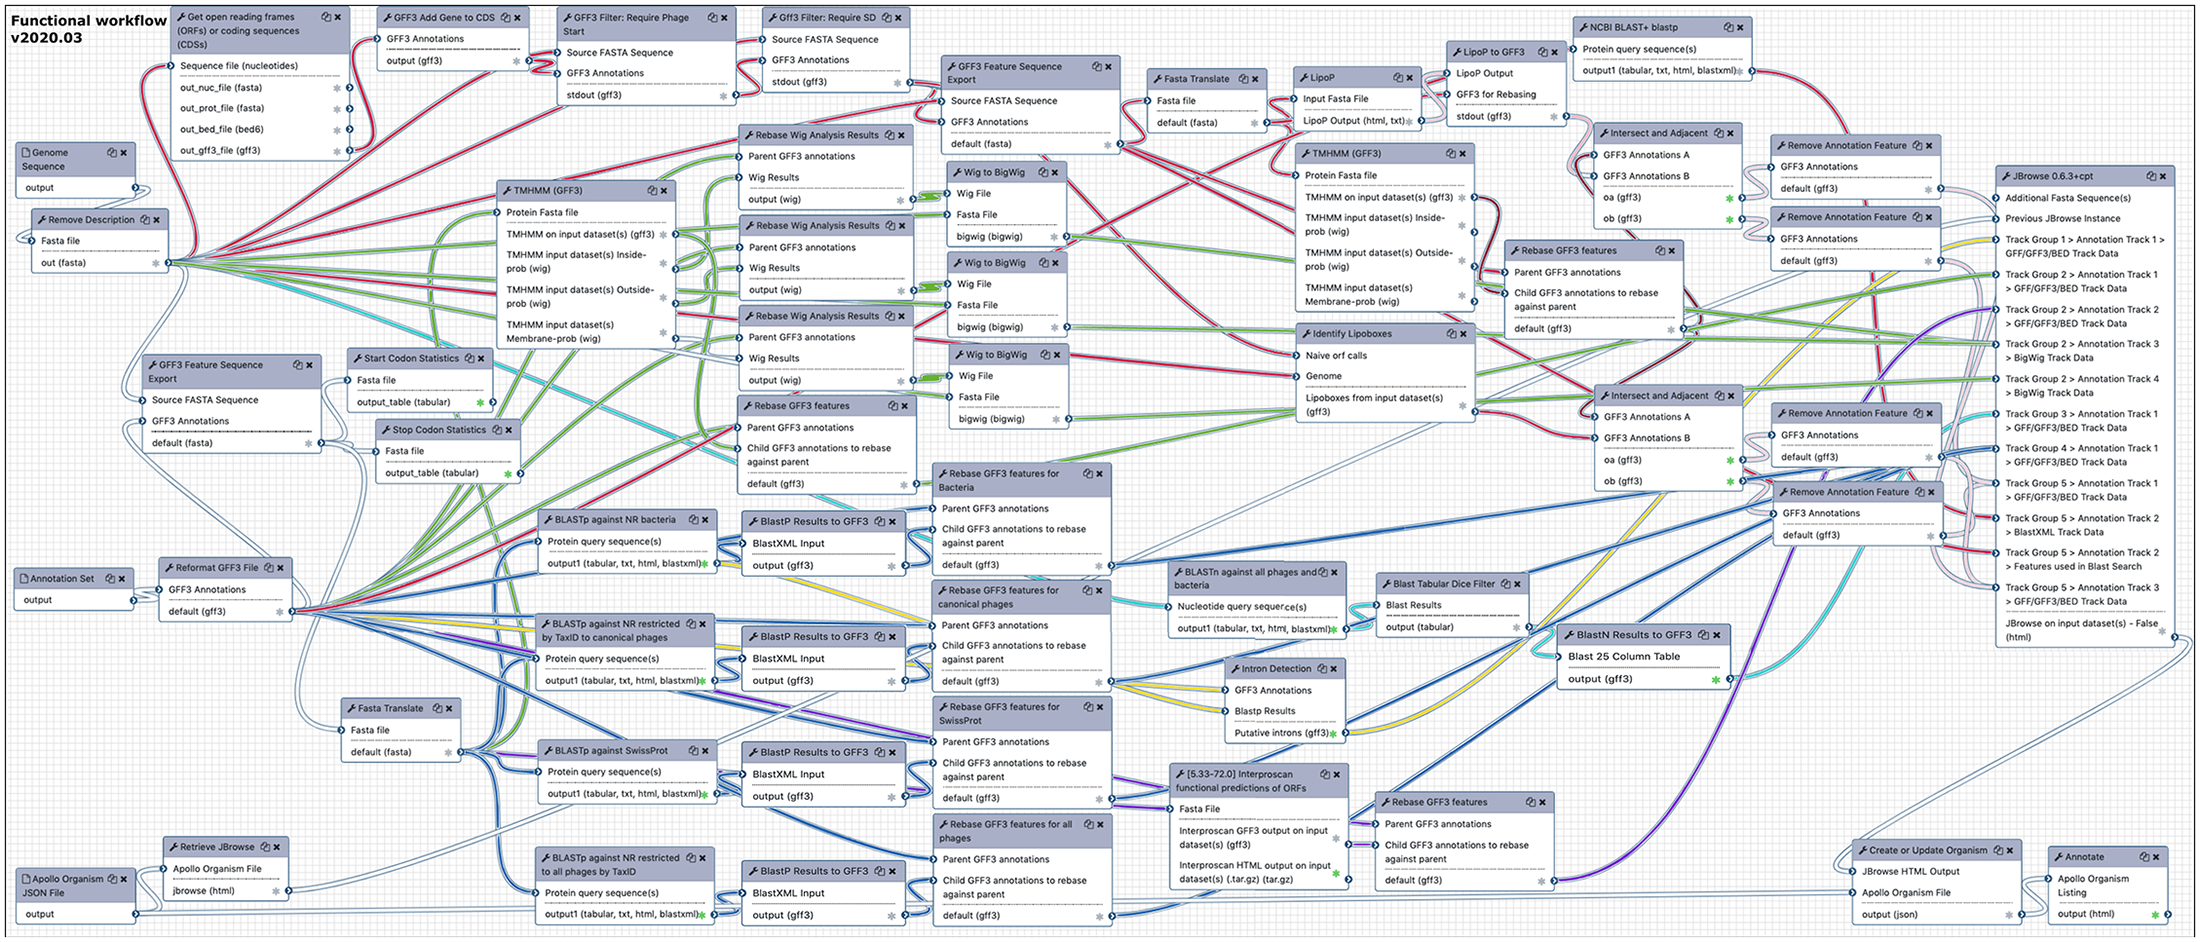
\includegraphics[width=\textwidth]{chapters/images/phages/3.png}
\caption{The functional workflow links tools in Galaxy used for
functional prediction.\\
Inputs for the functional workflow are gene calls paired with their
genome. These are piped through five sub-paths within the analysis. 1)
The BLASTn path uses full genomic nucleotide sequence (light blue
noodles). 2) The BLASTp protein analysis against curated (UniProtKB
SwissProt) and sequence-inclusive databases (NCBI nonredundant (nr))
(dark blue noodles). 3) The search for interrupted genes like introns
compiles separate CDS hits to the same protein (yellow noodles). 4) A
directed search for spanin proteins using TMHMM, lipobox-finding (using
LipoP and a motif search), and BLASTp against a curated database
(magenta and pink noodles). 5) Domain analysis plots comprehensive TMHMM
outputs and InterProScan results for conserved domains and signatures
(green and purple noodles, respectively).}\label{pcbi.1008214.g003}
}
\end{figure}

The independent segments of the workflow will be discussed in these
sections: BLAST analysis, InterProScan, and transmembrane domain finding
(the intron and spanin detection segments are described above). As an
added value feature, start and stop codon statistics are calculated.

\emph{BLAST}. First, the genome sequence is analyzed by BLASTn
(dc-megablast) with a 0.001 expectation cutoff, against the NCBI
nonredundant (nt) database restricted by all phages and bacterial
TaxIDs. The tabular BLASTn results are parsed with the \textbf{Blast
Tabular Dice Filter} tool (filters results with low Dice coefficient,
and requires 50--100\% identity), then mapped back onto the genome as a
GFF3 for display in JBrowse. Second, the CDS features in GFF3 format are
extracted from the structural annotation results, translated, and
analyzed in four separate jobs by traditional BLASTp at a 0.001
expectation value cutoff and default parameters. One job searches
against the UniProtKB SwissProt database, which includes only manually
annotated and reviewed sequences, providing a first good clue to their
function. Two BLASTp jobs search against the NCBI nr database restricted
to all phages and canonical phages
(\protect\hyperlink{pcbi.1008214.s003}{S3 Table}) by TaxID. The fourth
BLASTp analysis searches against the entire nr database. All BLASTp
outputs (in XML format) are converted to GFF3, then `rebased', or
mapped, back to the parent genome for display as an evidence track in
JBrowse format.

\emph{InterProScan} is a conserved domain search tool incorporating
information from several other services \cite{Quevillon_2005,Zdobnov_2001,Hunter_2009,Jones_2014}. In the CPT Galaxy
workflow, the same translated CDS features used for BLASTp analysis are
searched against conserved domain databases by InterProScan, which
returns a GFF3-formatted result that is mapped (or `rebased') back onto
the parent genome for JBrowse display.

\emph{Transmembrane domains} are predicted from the translated features
using TMHMM 2.0 \cite{Krogh_2001}. The simple output is a GFF3 file, which, when
displayed in Apollo shows the location of the probable TMD, and gives
its predicted orientation in the feature name. Three additional outputs
for inside, outside, and membrane probability are converted from wig to
bigwig format for a plot format display \cite{Kent_2010}, and mapped back onto
the parent GFF3 at the proper location. Additionally, transmembrane
domains and signal peptides are predicted by Phobius, which is
incorporated into the InterProScan software package \cite{Jones_2014,Kent_2010,K_ll_2004}.

The final output of the workflow is the direct Apollo link to the
updated JBrowse instance for the organism. In Apollo, each evidence
track will be displayed in context with the rest of the genome for
evaluation in functional prediction. After predictions are completed,
the genome annotations can be returned to Galaxy with the Retrieve Data
tool, yielding a FASTA and paired GFF3 file. These can then be converted
into the five-column table required by NCBI for deposition into Genbank,
as described elsewhere.

\subsection*{Comparative genomics workflow}

The goal of the comparative workflow is to identify the most related
phages to the query organism, compared at both nucleotide and protein
levels. This workflow requires the genomic DNA sequence in FASTA format
and the GFF3 annotations of protein-coding genes, and returns tables
listing the most related organisms by BLASTn and BLASTp analysis, and a
series of pairwise DNA dot plots. There are 11 steps in the comparative
workflow and it usually takes less than ten minutes to run
(\protect\hyperlink{pcbi.1008214.g004}{Fig 4}).

\begin{figure}
\hypertarget{pcbi.1008214.g004}{%
\centering
	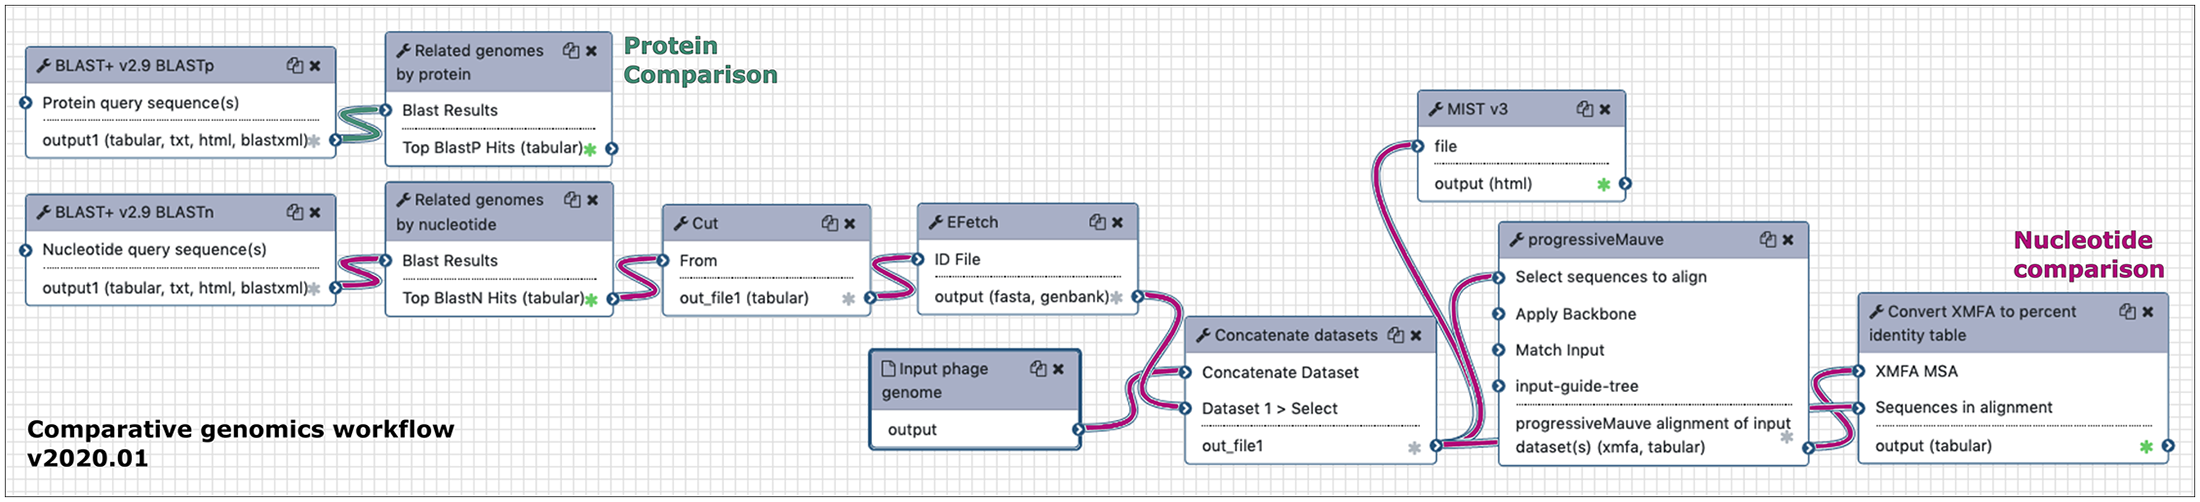
\includegraphics[width=\textwidth]{chapters/images/phages/4.png}
\caption{The comparative genomics workflow calculates nucleotide and
protein similarity to other phages.\\
The protein comparison branch starts with a BLASTp job against the nr
database, restricted by all phage TaxIDs (see full list in
\protect\hyperlink{pcbi.1008214.s003}{S3 Table}), and is then sorted
according to the organisms with the highest number of unique protein
hits (teal noodles). The nucleotide comparison branch begins with a
BLASTn job against the nt database, also restricted by all phage TaxIDs.
Top nucleotide hits are sorted based on dice score, which accounts for
the total coverage. The top five genome sequences are fetched from NCBI,
concatenated with the query genome and routed to MIST v3 for a dot plot,
and progressiveMauve for calculation of pairwise percent identity
(magenta noodles).}\label{pcbi.1008214.g004}
}
\end{figure}

Protein comparison is performed by a BLASTp search against NR restricted
by all phage TaxIDs (\protect\hyperlink{pcbi.1008214.s003}{S3 Table})
and an expectation value cutoff of 0.001. The top hits (default is 20)
are parsed from the custom tabular output by TaxID and returned as a
table with the phage common name, NCBI TaxID, and number of similar
unique proteins they share with the query phage.

Full-genome nucleotide comparison starts with a traditional BLASTn
megablast restricted to all phages in the NCBI nr database using a 0.001
expectation value cutoff. The number of user-specified top hits (default
is ten) are parsed from the custom tabular output based on percent
identity (calculated for the query:subject pair according to the Dice
coefficient = (2 * \# identical matches)/((genome 1 length) + (genome 2
length))). With this information, the full FASTA record for each top
matching genome is retrieved via the NCBI \textbf{EFetch} utility. After
concatenation, the related genomes are processed by \textbf{MIST} v3 to
generate a dot plot; MIST builds upon Gepard \cite{Krumsiek_2007} to generate a
matrix of multiple pairwise dot plots for a set of input sequences. The
MIST Python script calls Gepard for each pairwise comparison and builds
the combined image and image map. DNA sequences are also compared by
\textbf{progressiveMauve} v2.4.0, with the aligned blocks extracted and
output as a table with the \textbf{Convert XMFA to percent identity
table} tool, which presents overall percent nucleotide identity as a
Dice coefficient \cite{Krumsiek_2007,Darling_2010}.

The data in these tables can be directly used for publication, as
reference for finding literature on the genome type, or as the basis for
additional comparative genomics including the generation of synteny
plots using tools in CPT Galaxy like \textbf{X-Vis}, \textbf{Genome
Mapper}, or \textbf{EasyFig} \cite{Sullivan_2011}.

\subsection*{More on workflows}

The three workhorse workflows described can be customized in the Galaxy
workflow editor by addition or removal of individual tools, updating
tool functionality, or simply tweaking job parameters as needed. New
mainstay workflow versions we prepare regularly become publicly
available to the community, and users can contribute their
customizations or specialized workflows as well. The signature workflows
described above are geared towards the annotation of new genomes, but we
will note a few additional applications of the entire interface here.
Importantly, pre-annotated genomes can be loaded into Apollo using the
\emph{Upload Genbank into Apollo} (Genbank file input) or \emph{Upload
Previously Annotated Sequence to Apollo} (FASTA and GFF3 input)
workflows for updating by the user or community, as determined by whom
the user gives access to the organism. This will aid in our goal of
reaching at least one ``gold-standard'' annotated genome per
representative phage type. Users can also compare directly to the
original annotations by adding them as an evidence track with the
\emph{GFF3 to Apollo evidence track} workflow.

CPT Galaxy users have also built and shared a variety of generally
applicable routines. There is a whole collection of workflows that will
perform an analysis and push the results to an evidence track in Apollo,
usually BLAST jobs. The workflows \emph{Custom BLASTp to Apollo Evidence
Track--UserDB} and its variation from a \emph{Local DB} allow running a
BLASTp analysis against a user-generated local database. A specific use
case is the \emph{BLAST antiCRISPRdb to Apollo Evidence Track} workflow,
which searches against a local copy of the curated anti-CRISPRdb
\cite{Dong_2017}. Another useful workflow set, \emph{X-vis from GFF3/Fasta},
will generate a synteny map converting BLAST similarity into protein
XMFA format for visualization across the entire genome. The direct links
to current versions of the workflows mentioned here are listed in
\protect\hyperlink{pcbi.1008214.s004}{S4 Table}. A full list of the most
recent published versions for the annotation pipeline and all other
workflows can be accessed at
\url{https://cpt.tamu.edu/galaxy-pub/workflows/list_published}.

\section*{Results \& discussion}

\subsection*{Comparison to other available annotation tools}

Various groups host annotation systems publicly accessible for phage
annotation. DNAMaster is arguably the most widely used program for
teaching phage annotation in the undergraduate education context
\cite{Jordan_2014}. Thousands of students have performed phage annotation through
the SEA-PHAGES program in this stand-alone Windows program written
originally by Jeffrey Lawrence. Recently, an independent research group
released multiPhATE, a downloadable command-line bioinformatics pipeline
for functional annotation of phage isolates \cite{Ecale_Zhou_2019} One unique aspect in
multiPhATE is an accompanying tool designed specifically to detect phage
genes called PHANOTATE \cite{McNair_2019}.

Prior to these examples with adaptations tuned to phage annotation, most
automated pipelines in wide use were developed around prokaryotic
annotation needs. The service offered with deposit to Genbank, the
Prokaryotic Genome Annotation Pipeline (PGAP), is now available as a
stand-alone program for bacterial and archaeal genomes and used for all
RefSeq sequences \cite{Tatusova_2016,Haft_2017}. DFAST is a downloadable and web-based
prokaryotic genome annotation pipeline that boasts a 10-minute or less
processing time for full bacterial genomes \cite{Tanizawa_2017}. The RASTtk pipeline
is a downloadable and web-based prokaryotic genome annotation service,
used in the microbiology community as the basis for PATRIC (PAThosystems
Resource Integration Center) \cite{Aziz_2008,Overbeek_2013}. Their use of subsystems to
perform quick and automatic annotations has also been applied to phage
genome annotation, recently described in manual format \cite{McNair_2017}.

Given its widespread use, we compared the output of annotation with the
tools in CPT Galaxy to RASTtk for five phages representing all the major
morphotypes: four that we originally annotated, and phage T1 from RefSeq
(\protect\hyperlink{pcbi.1008214.s005}{S5 Table}). The final number of
genes called was similar, within six of each other, with CPT Galaxy
annotations always having the higher count. The phages annotated using
the CPT Galaxy-Apollo platform had fewer proteins without a functional
prediction (hypothetical or phage protein). Finally, the number of genes
called with a valid Shine-Dalgarno sequence was higher for CPT Galaxy,
but only by a maximum of seven genes in total. In addition to missing
more complex genome features, such as terminal repeat regions and
rho-independent terminators, RASTtk did not specifically assign function
to various known phage proteins with bioinformatically recognizable
characteristics, such as the spanins and translationally frameshifted
tape measure protein chaperones.

No currently available automated annotation algorithm can reasonably be
expected to reach the highest quality product that manual, human effort
can produce, and that in turn is inferior to empirical data to support
annotations. However, it is not always feasible to invest significant
researcher time on upstream annotation processes. While experienced
annotators can be quite efficient, when speed is of the essence,
automated pipelines can be combined with the convenient browsing and
editing tools available in the CPT Galaxy for polishing. Additionally,
the annotation can be performed collaboratively across groups or
institutions, making use of the ``Google Docs''-type functionality, as
we have done in several instances \cite{Marc_2019,Culbertson_2019,Freeman_2019}. Finally, the system's
application to a classroom setting is also immediately apparent, even a
virtual classroom, where teams can work on the same genome, and all
contributions are logged per user.

\section*{Conclusion}

Here, we have described a complete, easy-to-use web-based platform for
phage annotation. The powerful suite of tools housed in the CPT Galaxy
instance provides a dynamic, scalable framework for genome data analyses
that can be used independently of, or in conjunction with the community
genome editor, Apollo. In both research and educational contexts, the
CPT Galaxy and Apollo system allows users to focus on the biology behind
annotation rather than the minutiae of server maintenance, command-line
operations and file management. This is essential to allow us to use the
flood of sequencing data to move deeper into the understanding of phage
biology and the fundamental principles that govern their bacterial
hosts, and make informed decisions about their applications in the
future.

\section*{Acknowledgements}

The Center for Phage Technology received an Initial University
Multidisciplinary Research Initiative from Texas A\&M University and
Texas AgriLife. We are also grateful to the Texas A\&M Department of
Biochemistry and Biophysics for support. Many CPT staff, undergraduates
and graduate students in the BICH 464 Bacteriophage Genomics course of
the Department of Biochemistry and Biophysics at Texas A\&M have tested
the system through their use since the initiation of this project. We
thank Rodolfo Aramayo for early suggestions to implement Galaxy. We
thank the Galaxy community contributors for their development and
maintenance of this open resource, including the format of the training
materials. Additionally, we thank Suzanna Lewis and Nathan Dunn for
their support in adapting Apollo to phage annotation.


\footnotesize
\bibliographystyle{hexy.bst}
\bibliography{references}
\normalsize
